\subsection{Analyseklasser}
Inden analyseklasserne udarbejdes, foretages en analyse ud fra systembeskrivelsen, use case og funktionaliteter til at identificere substantiver og verber. Dette gøres for at sikre, at alle funktionaliteter indgår i klassediagrammet. Substantiver og verber fremgår af \autoref{tab:subverb}.

\begin{table}[H]
\centering
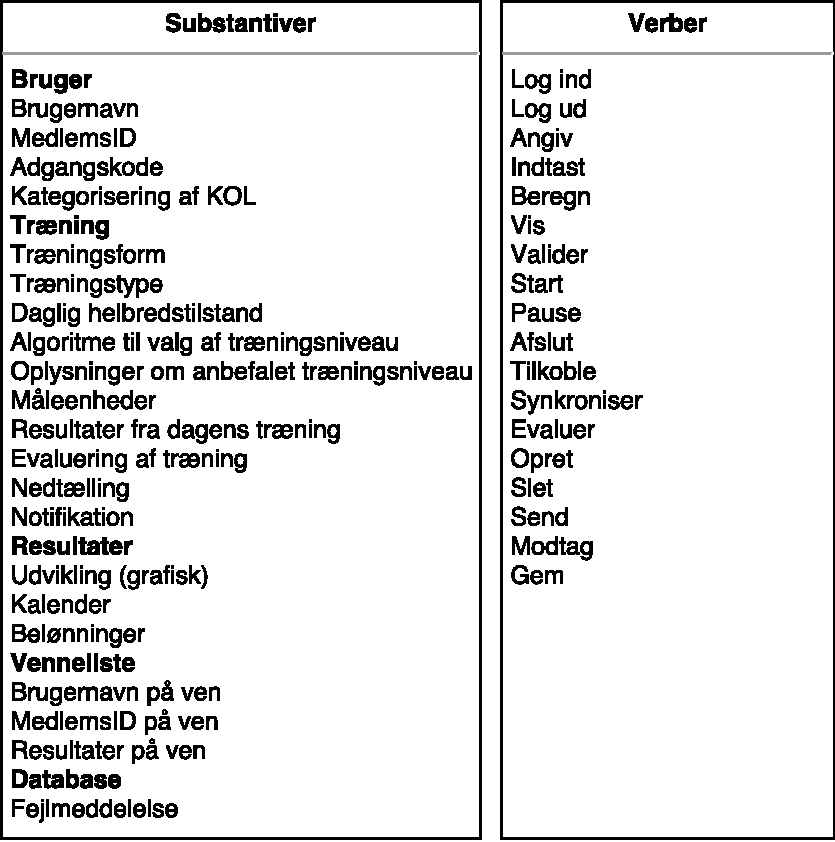
\includegraphics[width=1\textwidth]{figures/aktivitetsdiagram/substantiveverber}
\caption{Substantiver og verber identificeret ved analyse af systembeskrivelse, use case samt funktionaliteter.}
\label{tab:subverb}
\end{table}

\noindent
De fremhævede substantiver, brugeroplysninger, træning, resultater, venneliste og database, identificeres som klasser. Under hver klasse fremgår deres tilhørende attributter, der beskriver den overordnede klasse. Verberne betegner de metoder, der kan tilgås i de forskellige klasser. Klasserne er opstillet med relationer, hvilket fremgår af \autoref{fig:analyseklasse}.

\begin{figure}[H]
\centering
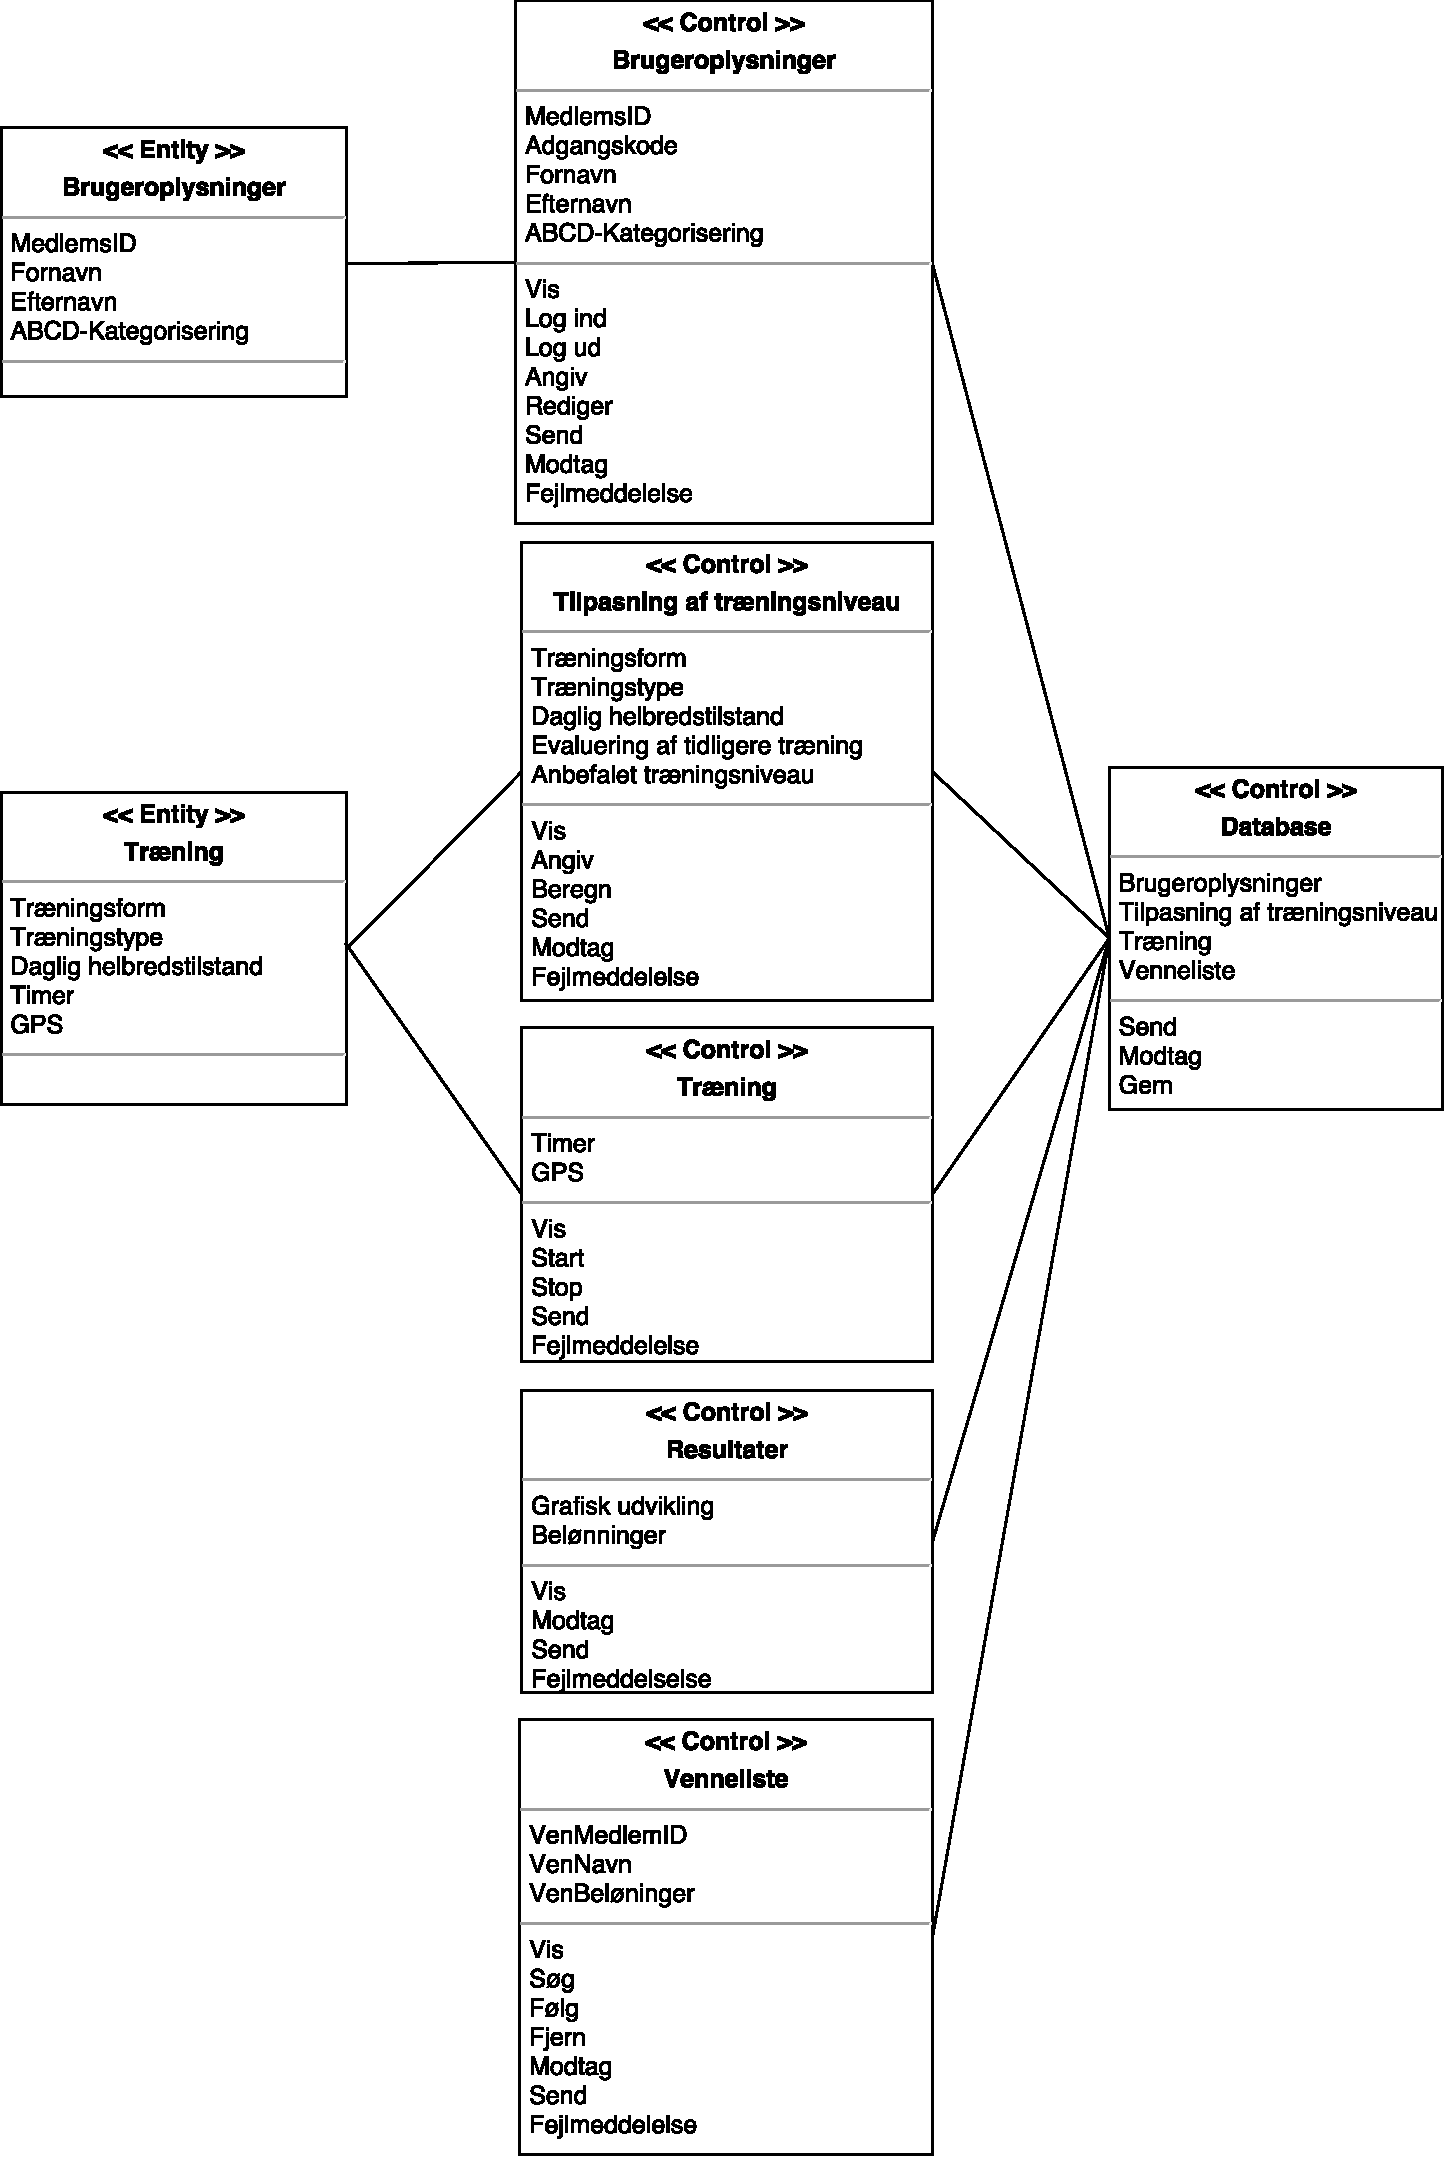
\includegraphics[width=1\textwidth]{figures/aktivitetsdiagram/analyseklasser}
\caption{Analyseklasser udarbejdet ud fra de identificerede substantiver og verber.}
\label{fig:analyseklasse}
\end{figure}

\noindent
Af \autoref{fig:analyseklasse} fremgår relationen mellem klasserne og deres dertilhørende attributter samt metoder. 

